\documentclass[12pt,oneside]{book}
\usepackage{geometry}                		% See geometry.pdf to learn the layout options. There are lots.
\geometry{a4paper}                   			% ... or a4paper or a5paper or ... 
%\geometry{landscape}                		% Activate for for rotated page geometry
%\usepackage[parfill]{parskip}    		% Activate to begin paragraphs with an empty line rather than an indent
\usepackage{graphicx}				% Use pdf, png, jpg, or epsß with pdflatex; use eps in DVI mode
								% TeX will automatically convert eps --> pdf in pdflatex		
\usepackage{amssymb}

\usepackage[spanish]{babel}			% Permite que partes automáticas del documento aparezcan en castellano.
\usepackage[utf8]{inputenc}			% Permite escribir tildes y otros caracteres directamente en el .tex
\usepackage[T1]{fontenc}				% Asegura que el documento resultante use caracteres de una fuente apropiada.

\usepackage{hyperref}				% Permite poner urls y links dentro del documento

\title{Mi Juego Favorito}
\author{Javier Tibau}
%\date{}							% Activate to display a given date or no date

\begin{document}
\maketitle
\tableofcontents

\chapter{Introducción}
El libro a continuación es creado como una herramienta para el desarrollo de habilidades de edición colaborativa de documentos de texto plano. La herramienta que habilita dicha colaboración, en este taller, es Git pero podría ser reemplazada por otros sistemas de versionamiento.

\chapter{Los Juegos}

\include{juegos/Buscaminas}
\include{juegos/Dota2}
\include{juegos/Zelda}
\section{Twisted Metal: }

\begin{figure}[htbp]
\begin{center}
\includegraphics[width=.60\textwidth]{./imagenes/skyward.jpg}
\caption{Zelda: Skyward Sword}
\label{Zelda: Skyward Sword}
\end{center}
\end{figure}
Zelda: Skyward Sword\footnote{\url{http://zelda.com/skywardsword/}} es el primer Zelda en ofrecerte total control de la espada y escudo via wiimote + nunchuck. Fue publicado en Noviembre del 2011 y ha sido uno de los juegos de Zelda más controversiales por su único modo de jugarlo con controles de movimiento.

La premisa del juego es que eres un chico (Link) que vive en una comunidad en una isla flotante y debes emprender un viaje a la superficie (Hyrule) para rescatar a Zelda.

\subsubsection{¿Por qué es uno de mis juegos favoritos?}
\begin{itemize}
\item[Gianni Carlo] Las reglas del juego son similares a los anteriores juegos de Zelda con el agregado que ahora cada enemigo fue diseñado con los controles de moviemiento en mente, no basta con agitar de izquierda a derecha el control para poder pasar el juego, y esto ayuda en gran parte a sumergirte en el juego ya que debes atacar de cierta forma a los enemigos y/o repeler ataques con tu escudo en el momento preciso sino recibes una penalidad. A pesar de esto, el juego no es atractivo para todo el mundo debido a la única opción de controles a los que alegan que no responden con suficiente precisión o a veces ni responden. Para mi, el gran interés del juego, aparte de presentar el origen de la historia del universo de Zelda, es el nuevo estilo de jugarlo y la experiencia de inmersión única que presenta a cualquier fan de la serie (los motion controls de Twilight Princess para Wii no cuentan en mi opinión ya que eran tan solo un test para ver que tan buena sería la acogida para implementarlo como única opción en el siguiente Zelda).
\end{itemize}
\section{Mortal Kombat Armageddon}

\begin{figure}[htbp]
\begin{center}
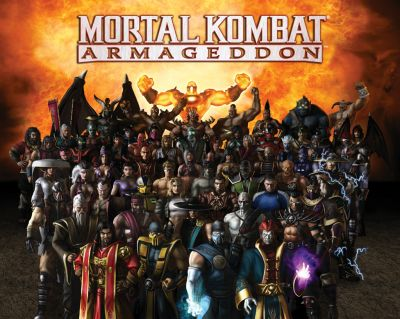
\includegraphics[width=.60\textwidth]{./imagenes/MortalK.jpg}
\caption{Mortal Kombat Armageddon}
\label{Mortal Kombat Armageddon}
\end{center}
\end{figure}

Mortal Kombat: Armageddon \footnote{\url{http://www.mortalkombat.net/armageddon/}} es un videojuego de la saga Mortal Kombat desarrollada por Midway Games. Este juego es una continuación directa de Mortal Kombat: Deception. El juego distribuyo más de 2 millones de copias por todo el mundo.
Las plataformas designadas para este juego son PlayStation 2 y Xbox en el 2006 y Wii en el 2007.

\subsubsection{¿Por qué es uno de mis juegos favoritos?}
\begin{itemize}
\item[Joao Sanga] Me gusta mucho por los gráficos, el modo de pelea y la historia. Las peleas en Mortal Kombat siempre conservarán su puntito gore (sangriento): sin él, nada diferenciaría a la saga de otros tantos juegos de lucha.
Aprendiendo de la experiencia en títulos pasados, MK Armageddon ha suavizado los controles, y ha ordenado todos los elementos en un sencillo menú. Pero la mecánica del juego sigue siendo la misma: cada luchador tiene dos métodos de combate –una técnica cuerpo a cuerpo, y lucha con arma-, junto con los clásicos combos aéreos, encadenados, llaves y contras. Quienes busquen un título de machaque fácil pulsando botones a toda velocidad, lo tienen complicado de nuevo: en Mortal Kombat los combates no lo parecen, SON lentos, ni de lejos tan vertiginosos como en cualquier juego de lucha de Namco. Los kombatientes se mueven en ocasiones como marionetas que responden mecánicamente a nuestras teclas.
En conclusión, Mortal Kombat Armageddon es uno de los mejores creados de la saga de Mortal Kombat.
\end{itemize}
\section{Gatos Gemelos}

\begin{figure}[htbp]
\begin{center}
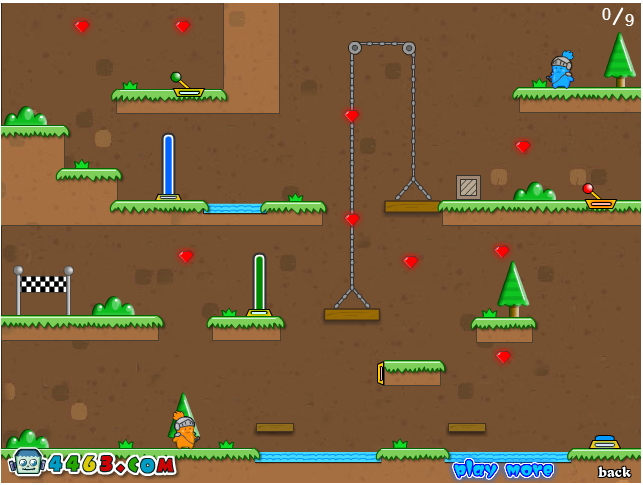
\includegraphics[width=.60\textwidth]{./imagenes/gatos1.png}
\caption{Gatos Gemelos}
\label{Gatos Gemelos}
\end{center}
\end{figure}
Gatos Gemelos \footnote{\url{http://ar.yayoye.com/twin-cat-online-game/22643/}} es un Juego en el que se deben mover a los personajes por la pantalla, como su nombre mismo lo dice son unos gatos gemelos, con los que iremos tratando de recoger diamantes y de lograr que interactúen entre ellos para superar los obstáculos.

\subsubsection{¿Por qué es uno de mis juegos favoritos?}
\begin{itemize}
\item[Tania Sánchez] En realidad no soy de esas personas que se vician con los juegos pero me llaman mucho la atención el tipo de juego que estimula el aprendizaje, me parece que este juego lo hace, ya que es un juego que se realiza en pareja en el que enseña el trabajo en equipo, a medida que avanzan los niveles va aumentando la dificultad del mismo, poniendo al usuario cada vez a pensar más en como vencer los obstaculos tomando en cuenta que un jugador debe ir a la par con el otro e irlo ayudando para juntos llegar a la meta, la dificultad del juego aparte de resolver como se debe avanzar, está en no olvidarse del compañero ya que aunque llegue uno de los dos solo a la meta no implicará que se pasará al siguiente nivel sino que deben llegar los dos juntos. 
\\
\\
Éste es un juego orientado más para niños pequeños para estimular el desarrollo intelectual y enseñarles el trabajo en equipo =).
\end{itemize}



\chapter{Conclusiones}
Cuales juegos fueron más populares y un breve razonamiento del porqué.

\end{document}  
